\subsection{Results}
\label{Results2}
\setlength{\parindent}{20pt}
\justifying

\subsubsection{\large{\emph{Participants}}}
\label{Exp2_ParticipantExclusion}

\noindent
One hundred and ninety one participants completed the experiment. Seven participants were then excluded for the following reasons: having a very slow mean testing response time (mean = 1986ms, n = 1 participant), having a very fast mean testing response time (mean = 175ms, n = 1), declaring to have filmed the training phase to help performance in testing (n = 1), having never responded ``yes'' in testing (n = 1), and having always responded ``yes'' in testing (n = 3). Therefore, data from 184 participants were analysed. This sample counted 93 males, and had a mean age of 22.22 years.

\subsubsection{\large{\emph{Group-level analyses}}}

\noindent
\underline{Familiarity test}

\noindent
This experiment also saw mean familiarity test scores significantly above chance (t(183) = 10.2, p$<$ 2.2e$^{-16}$) at 57\%. While the mean scores were comparable to experiment 1, responses in this phase were 40ms quicker than in experiment 1, indicating a better grasp of the material.

\begin{figure}[!htbp]
    \begin{center}
        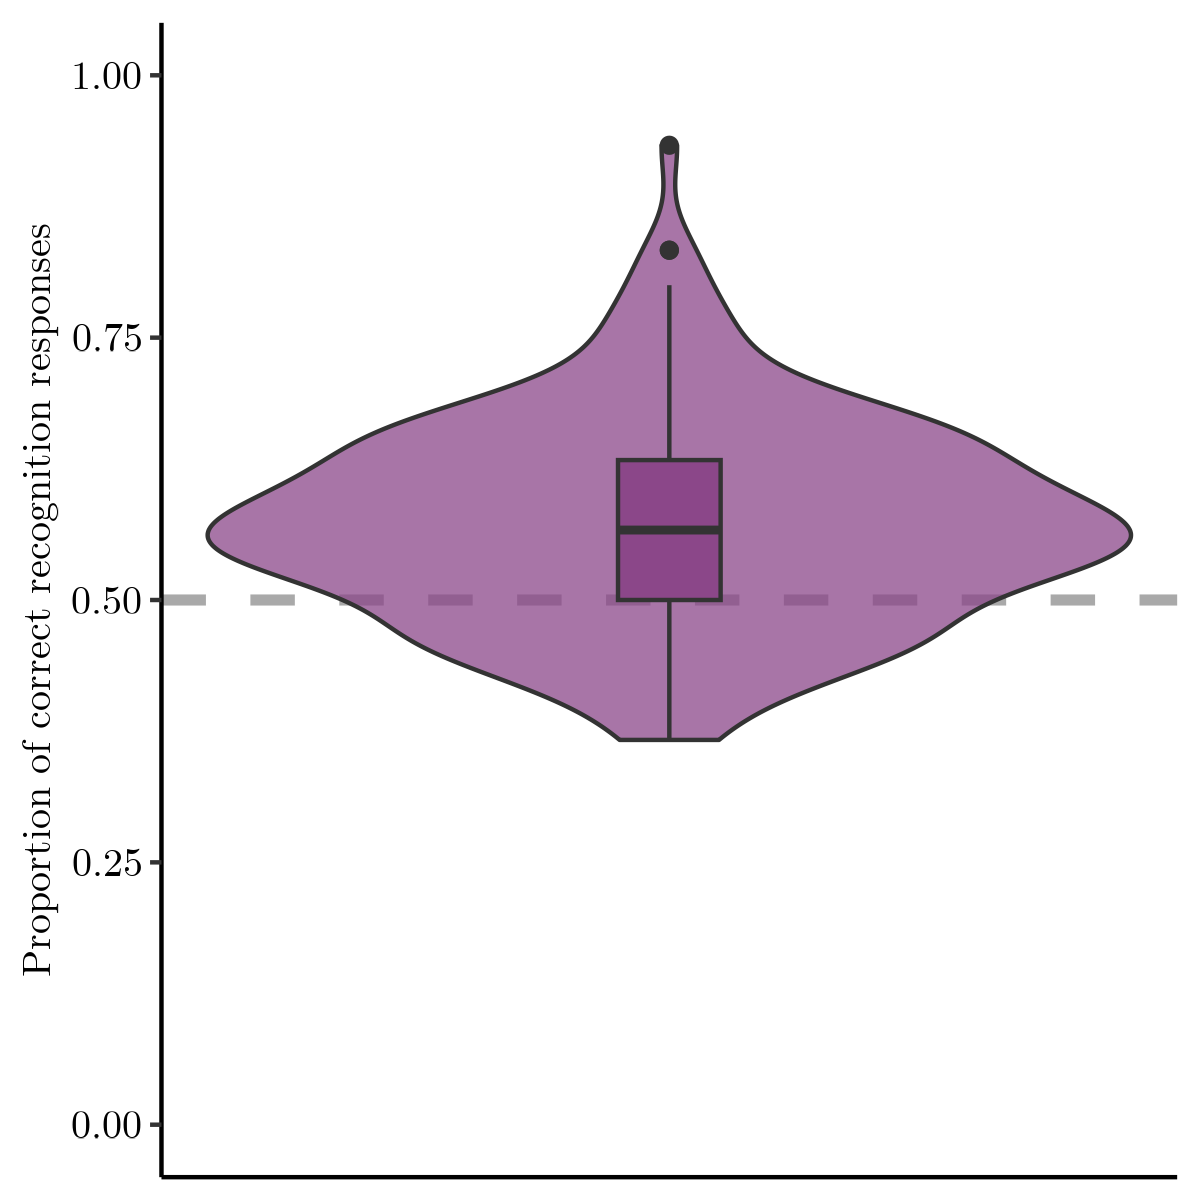
\includegraphics[width=0.6\textwidth]{Figures/exp2_familiarity_violinplt.png}
    \end{center}
    \caption[]{\justifying Violin plot and boxplot of the accuracy of familiarity test responses. The dashed line indicates chance level.}
    \label{exp2_familiarity}
\end{figure}

\noindent
\underline{Morpheme familiarity test}

\noindent
Results from experiment 1 were successfully replicated, with the morpheme familiarity effect also being present in experiment 2. Significant differences were found between the 0M (model intercept), 1M, and 2M conditions after linear modelling: Intercept $\beta$ = 0.09, z = 1.74, p = 0.08; 1M $\beta$ = 0.25, z = 5.81, p = 6.30e$^{-9}$; 2M $\beta$ = 0.55, z = 10.77, p = 5e$^{-27}$. Participants confronted with the 1M condition responded ``yes'' 6\% more than in the 0M condition (0M model fit = 0.52, SE = 0.01; 1M model fit = 0.58, SE = 0.01). The 2M condition attracted 7\% more ``yes'' responses than the 1M condition (2M model fit = 0.65, SE = 0.01). This pattern of results replicates that found in experiment 1.

\begin{figure}[!htbp]
    \begin{center}
        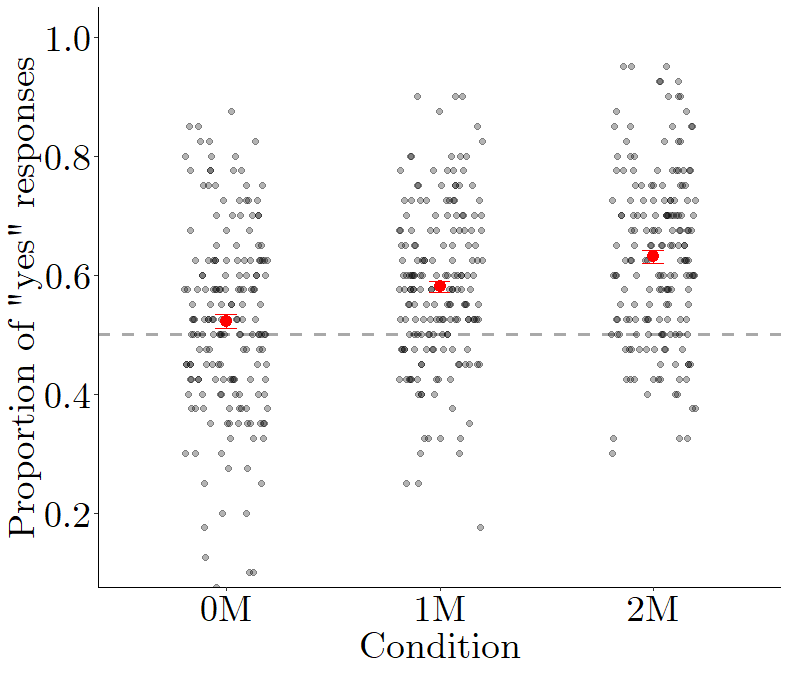
\includegraphics[width=0.6\textwidth]{Figures/Exp2_yes_allconditions.png}
    \end{center}
    \caption[]{\justifying Proportion of ``yes'' responses in each testing condition. The dashed line indicates chance level. The red circle shows the group mean, with bars as the standard error of the mean.}
    \label{exp2_morphfam}
\end{figure}

\noindent
\underline{2M performance}

\noindent
However, mean 2M accuracy was still not significantly different from chance: t(183) = -0.81, p = 0.42. In this version of the experiment, the mean d-prime score was -0.03, with an average c of -0.35, still showing no co-occurrence learning despite a clear bias towards ``yes'' in the 2M condition.

\begin{figure}[!htbp]
    \begin{center}
        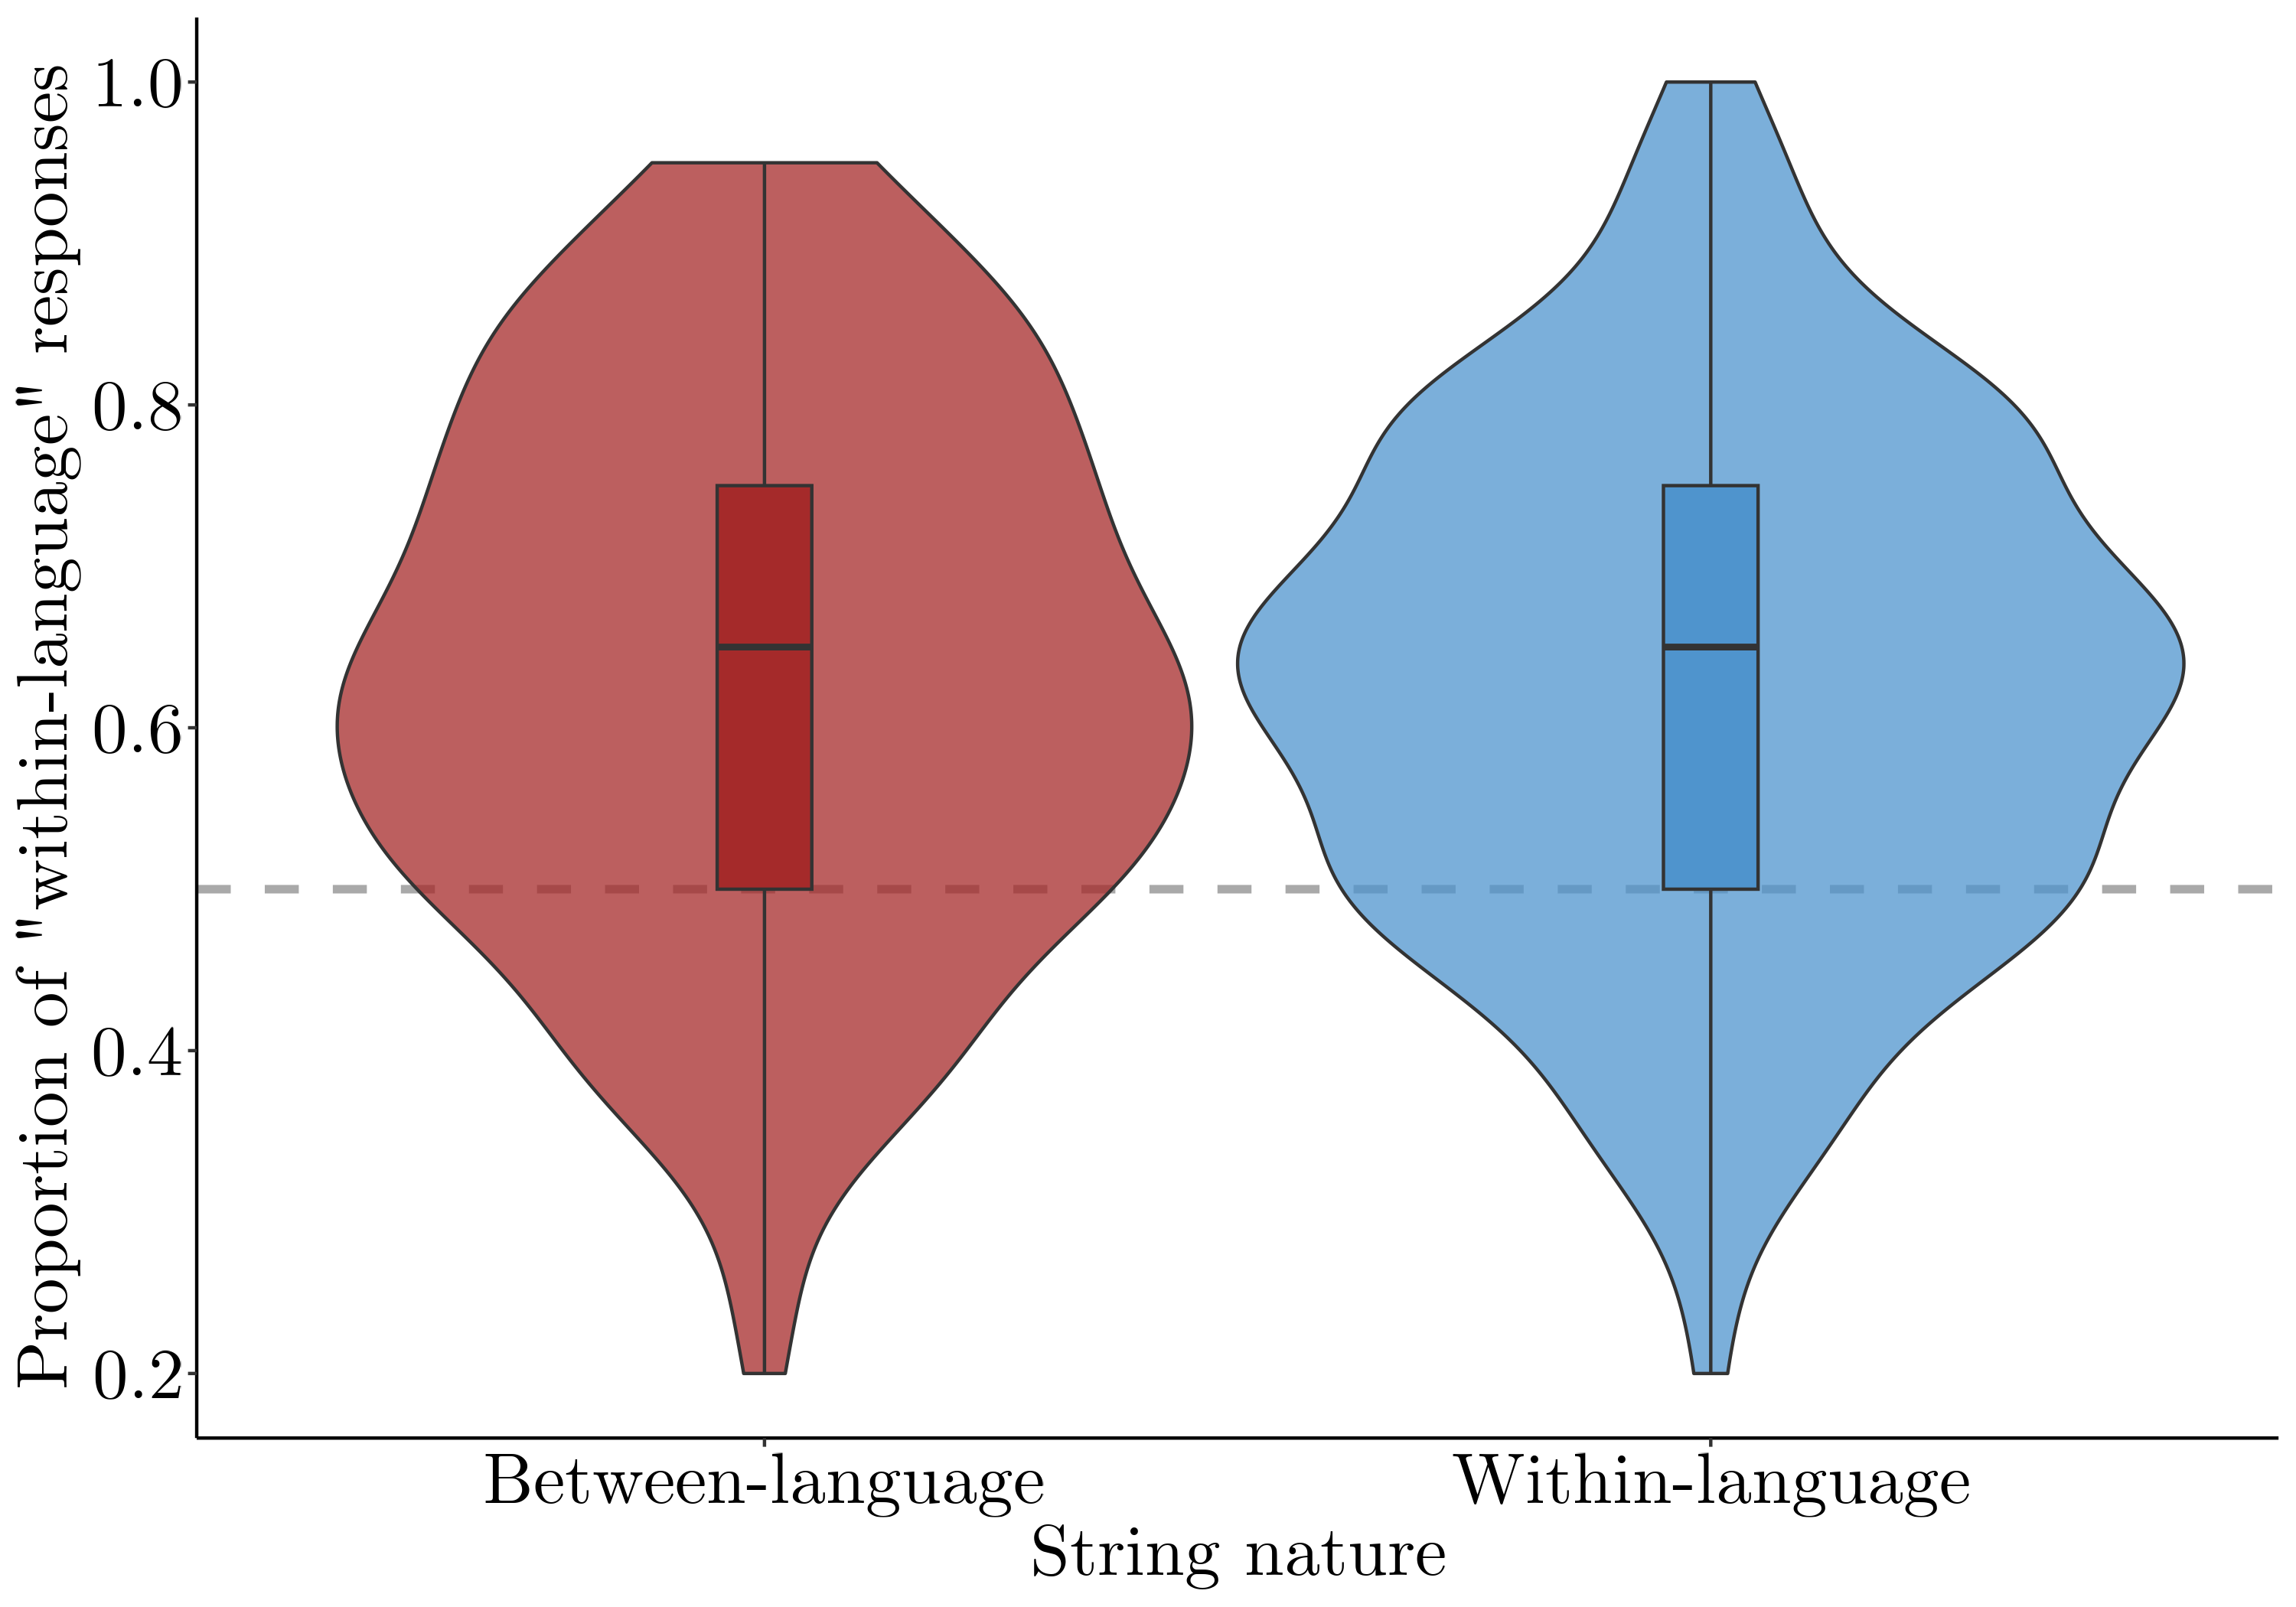
\includegraphics[width=0.6\textwidth]{Figures/exp2_2M_responses.png}
    \end{center}
    \caption[]{\justifying Boxplots of the proportion of ``within-language'' responses to each 2M combination type. The dashed line indicates chance level.}
    \label{exp2_2Mresponses}
\end{figure}

\subsubsection{\large{\emph{Individual differences analyses}}}

\noindent
\underline{BLP}

\noindent
Twenty-two participants completed the BLP for just one language, 70 did so for two languages, 51 for three, and 41 for four languages. English was the most dominant language, being the top L1 and L2 reported by participants. German was the most common L3 language, and Spanish was the most common L4. The languages declared by participants belonged to a total of 11 language families, with 20 unique branches. In this version of the experiment, 156 participants were same script multilinguals, and 28 were different script multilinguals.

\noindent
\underline{PCA}

\noindent
The PCA conducted on experiment 2 data produced five interesting PCs. PC1 loaded L4 components, and represented 20\% of the variance in the sample (the equivalent of PC9 from experiment 1). PC3 explained 17\% of the variance by representing L3 information (like PC1 in experiment 1). PC2 presented the contrast between L1 and L2 language use, with L1 use strongly negatively weighted, and L2 use strongly positively weighted (also like experiment 1's PC2). PC7 was for the L2 history measure (5\% of variance), replacing PC8 in experiment 1 logging the same variable. Finally, in an interesting deviation from experiment 1, no L2 proficiency measure was kept by the PCA in experiment 2, which instead placed value on PC9 storing L4 use (5\% of variance).

\noindent
\underline{Familiarity test}

\noindent
The PC component 9 dealing with L4 use was the only measure to significantly affect familiarity test accuracy: $\beta$ = -0.07, z = -2.30, p = 0.02.

\begin{figure}[!htbp]
    \begin{center}
        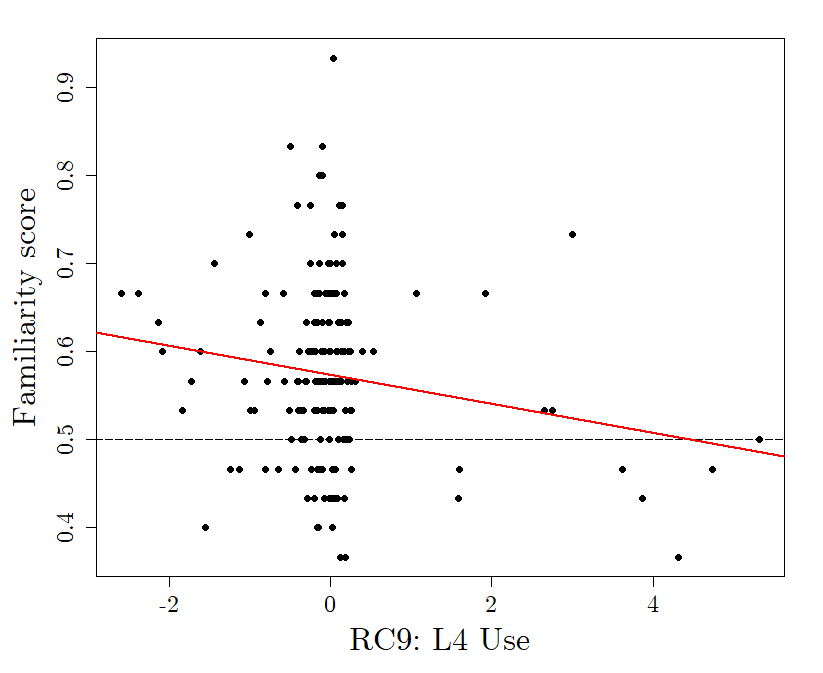
\includegraphics[width=0.50\textwidth]{Figures/Exp2_fam_PC9.png}
    \end{center}
    \caption[]{\justifying Familiarity test performance according to PC9 for L4 use, with model regression line in red. The dashed line at 0.5 indicates chance level.}
    \label{exp2_famanalyses}
\end{figure}

\noindent
\underline{Morpheme familiarity effect}

\noindent
Several variables influenced the overall proportion of ``yes'' responses across all testing conditions. These were the PC7 for L2 history ($\beta$ = 0.11, z = 2.20, p = 0.03), bilingual balance (L1-L2 difference; $\beta$ = -0.10, z = -2.02, p = 0.04), and multilingual experience ($\beta$ = 0.15, z = 3.34, p = 0.0008). 

As compared with the 0M condition, multilingual experience also had a significant interaction effect on 1M ``yes'' responses ($\beta$ = -0.08, z = -2.26, p = 0.02). The amount of ``yes'' answers to the 1M condition was also influenced by cosine similarity (1M*cosine similarity interaction: $\beta$ = 1.72, z = 2.05, p = 0.04), with increased multilingual balance meaning greater preference for novel 1M combinations when compared to 0M responses.

\begin{figure}[!htbp]
    \begin{minipage}{0.49\linewidth}
        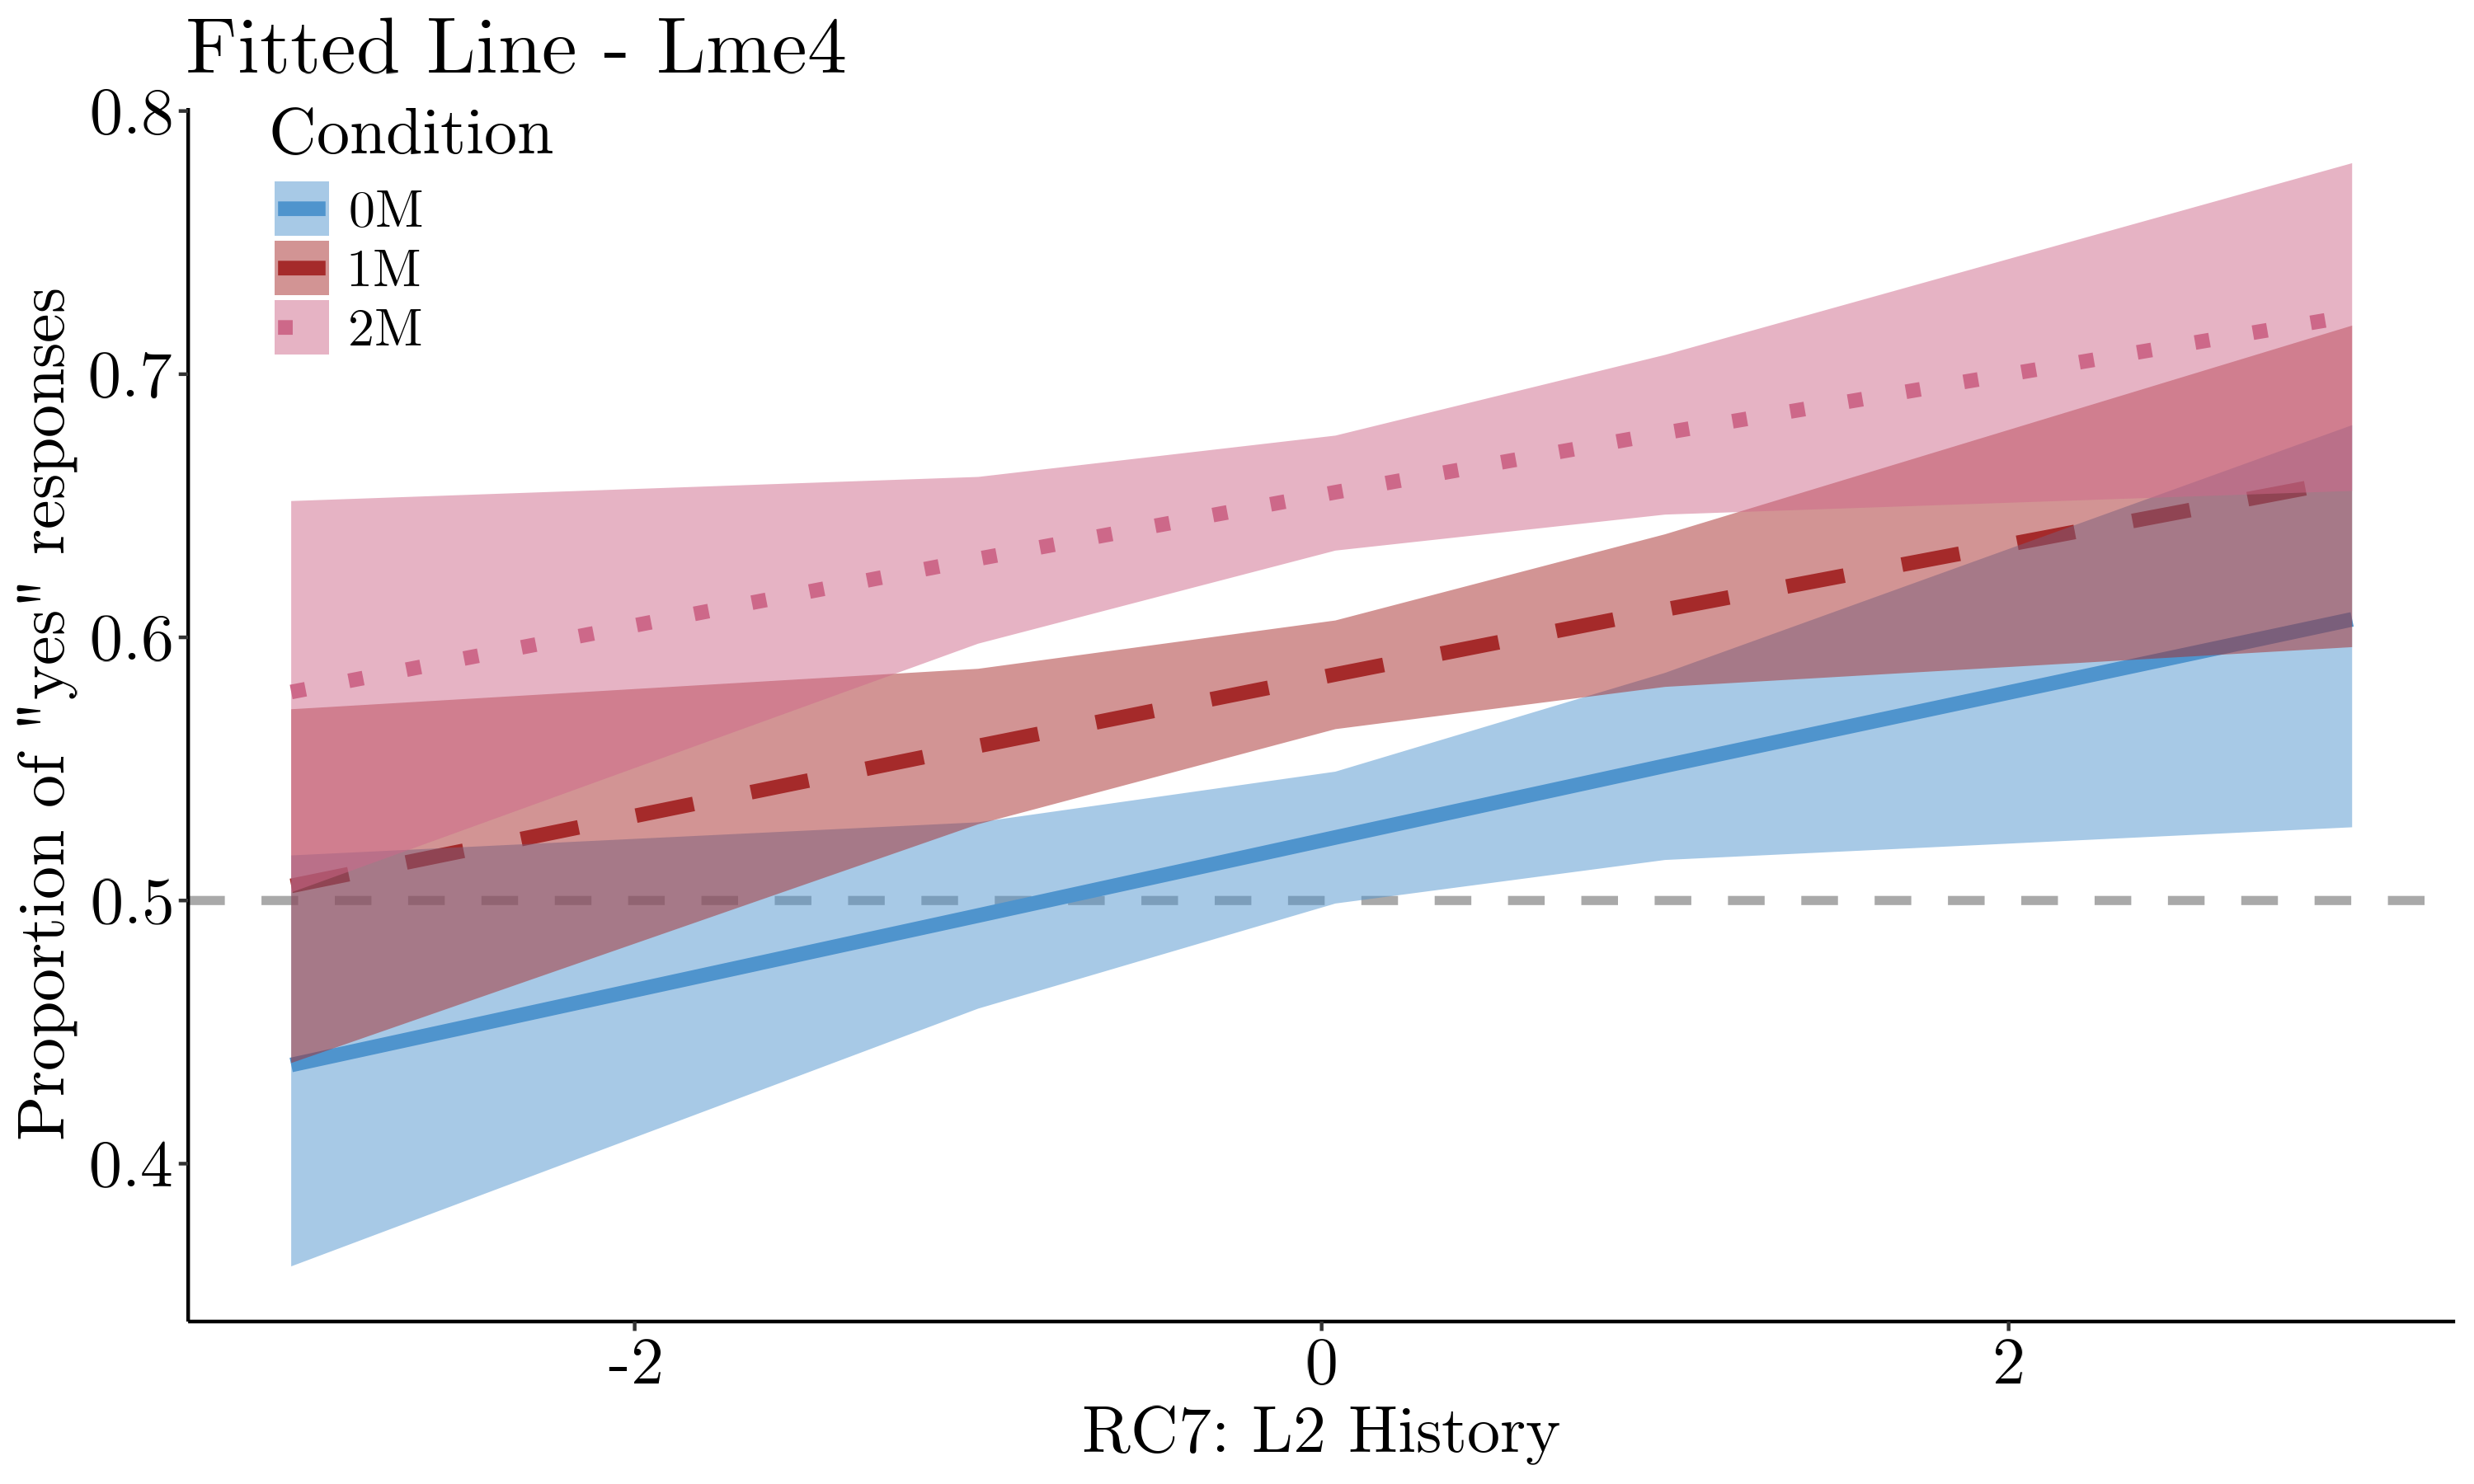
\includegraphics[width=0.99\textwidth]{Figures/Exp2_yes_PC7.png}
    \end{minipage}
    \begin{minipage}{0.49\linewidth}
        \centering
        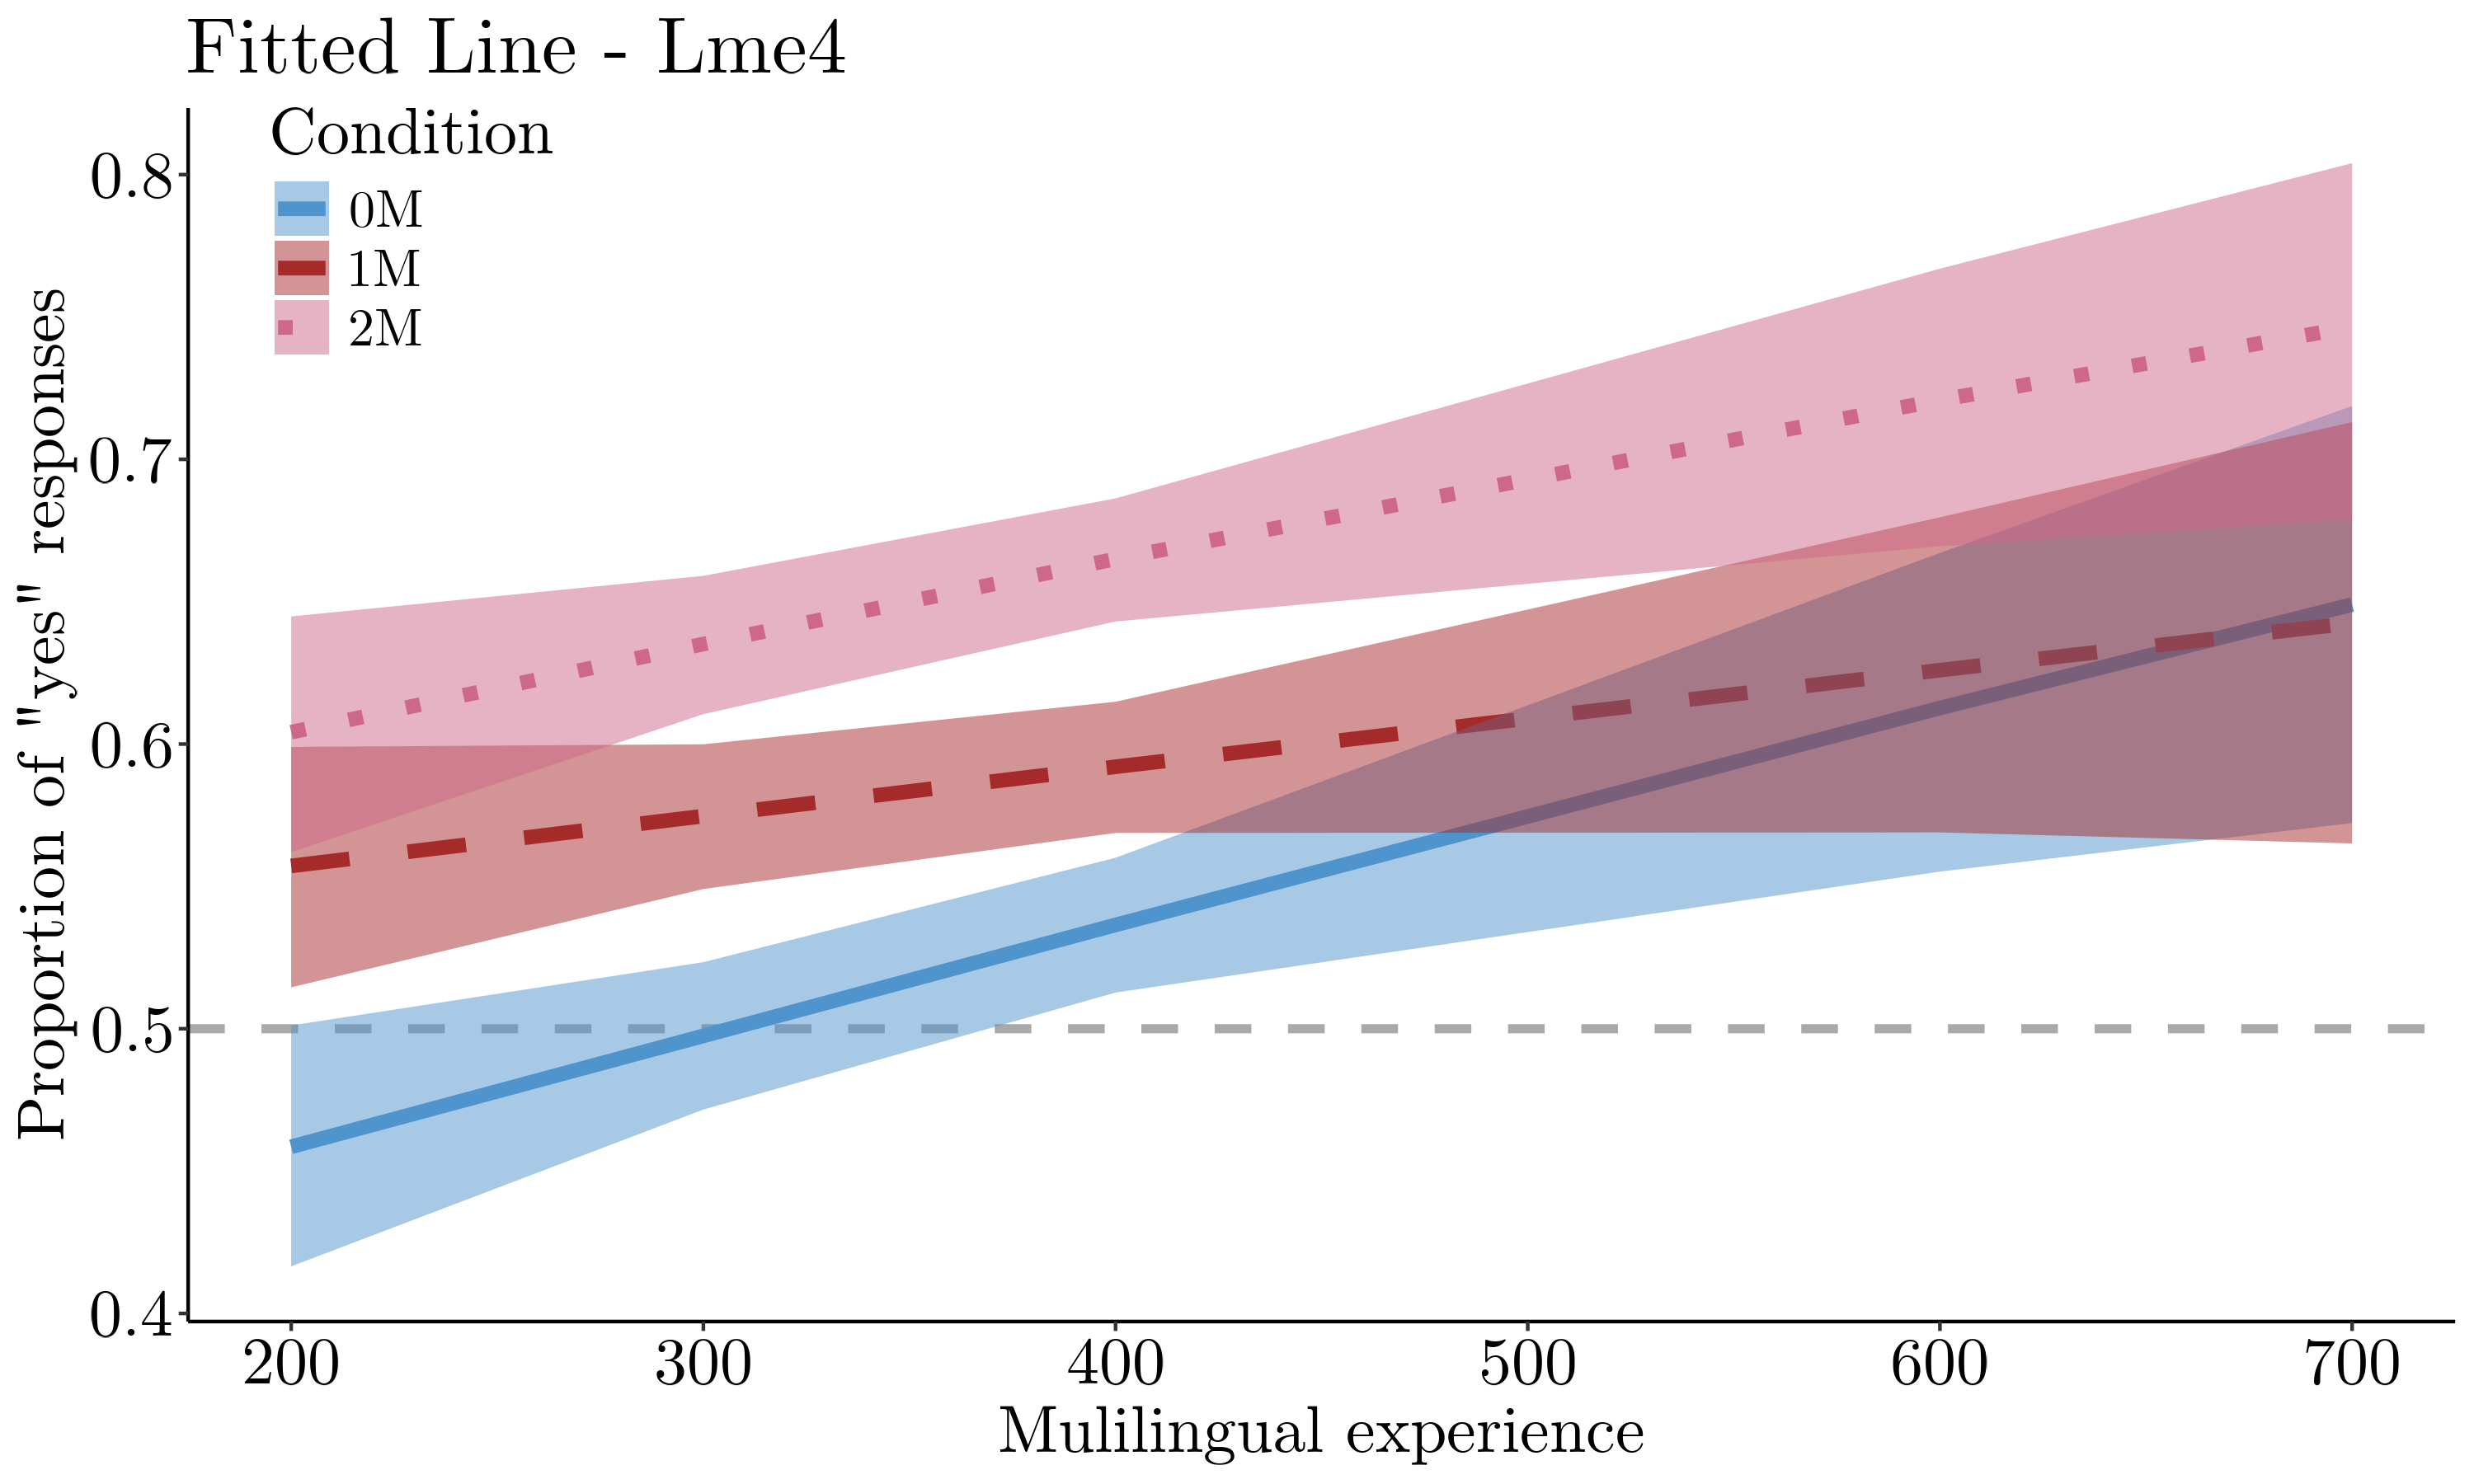
\includegraphics[width=0.99\textwidth]{Figures/Exp2_yes_multiexp.png}
    \end{minipage}
    \begin{minipage}{0.49\linewidth}
        \centering
        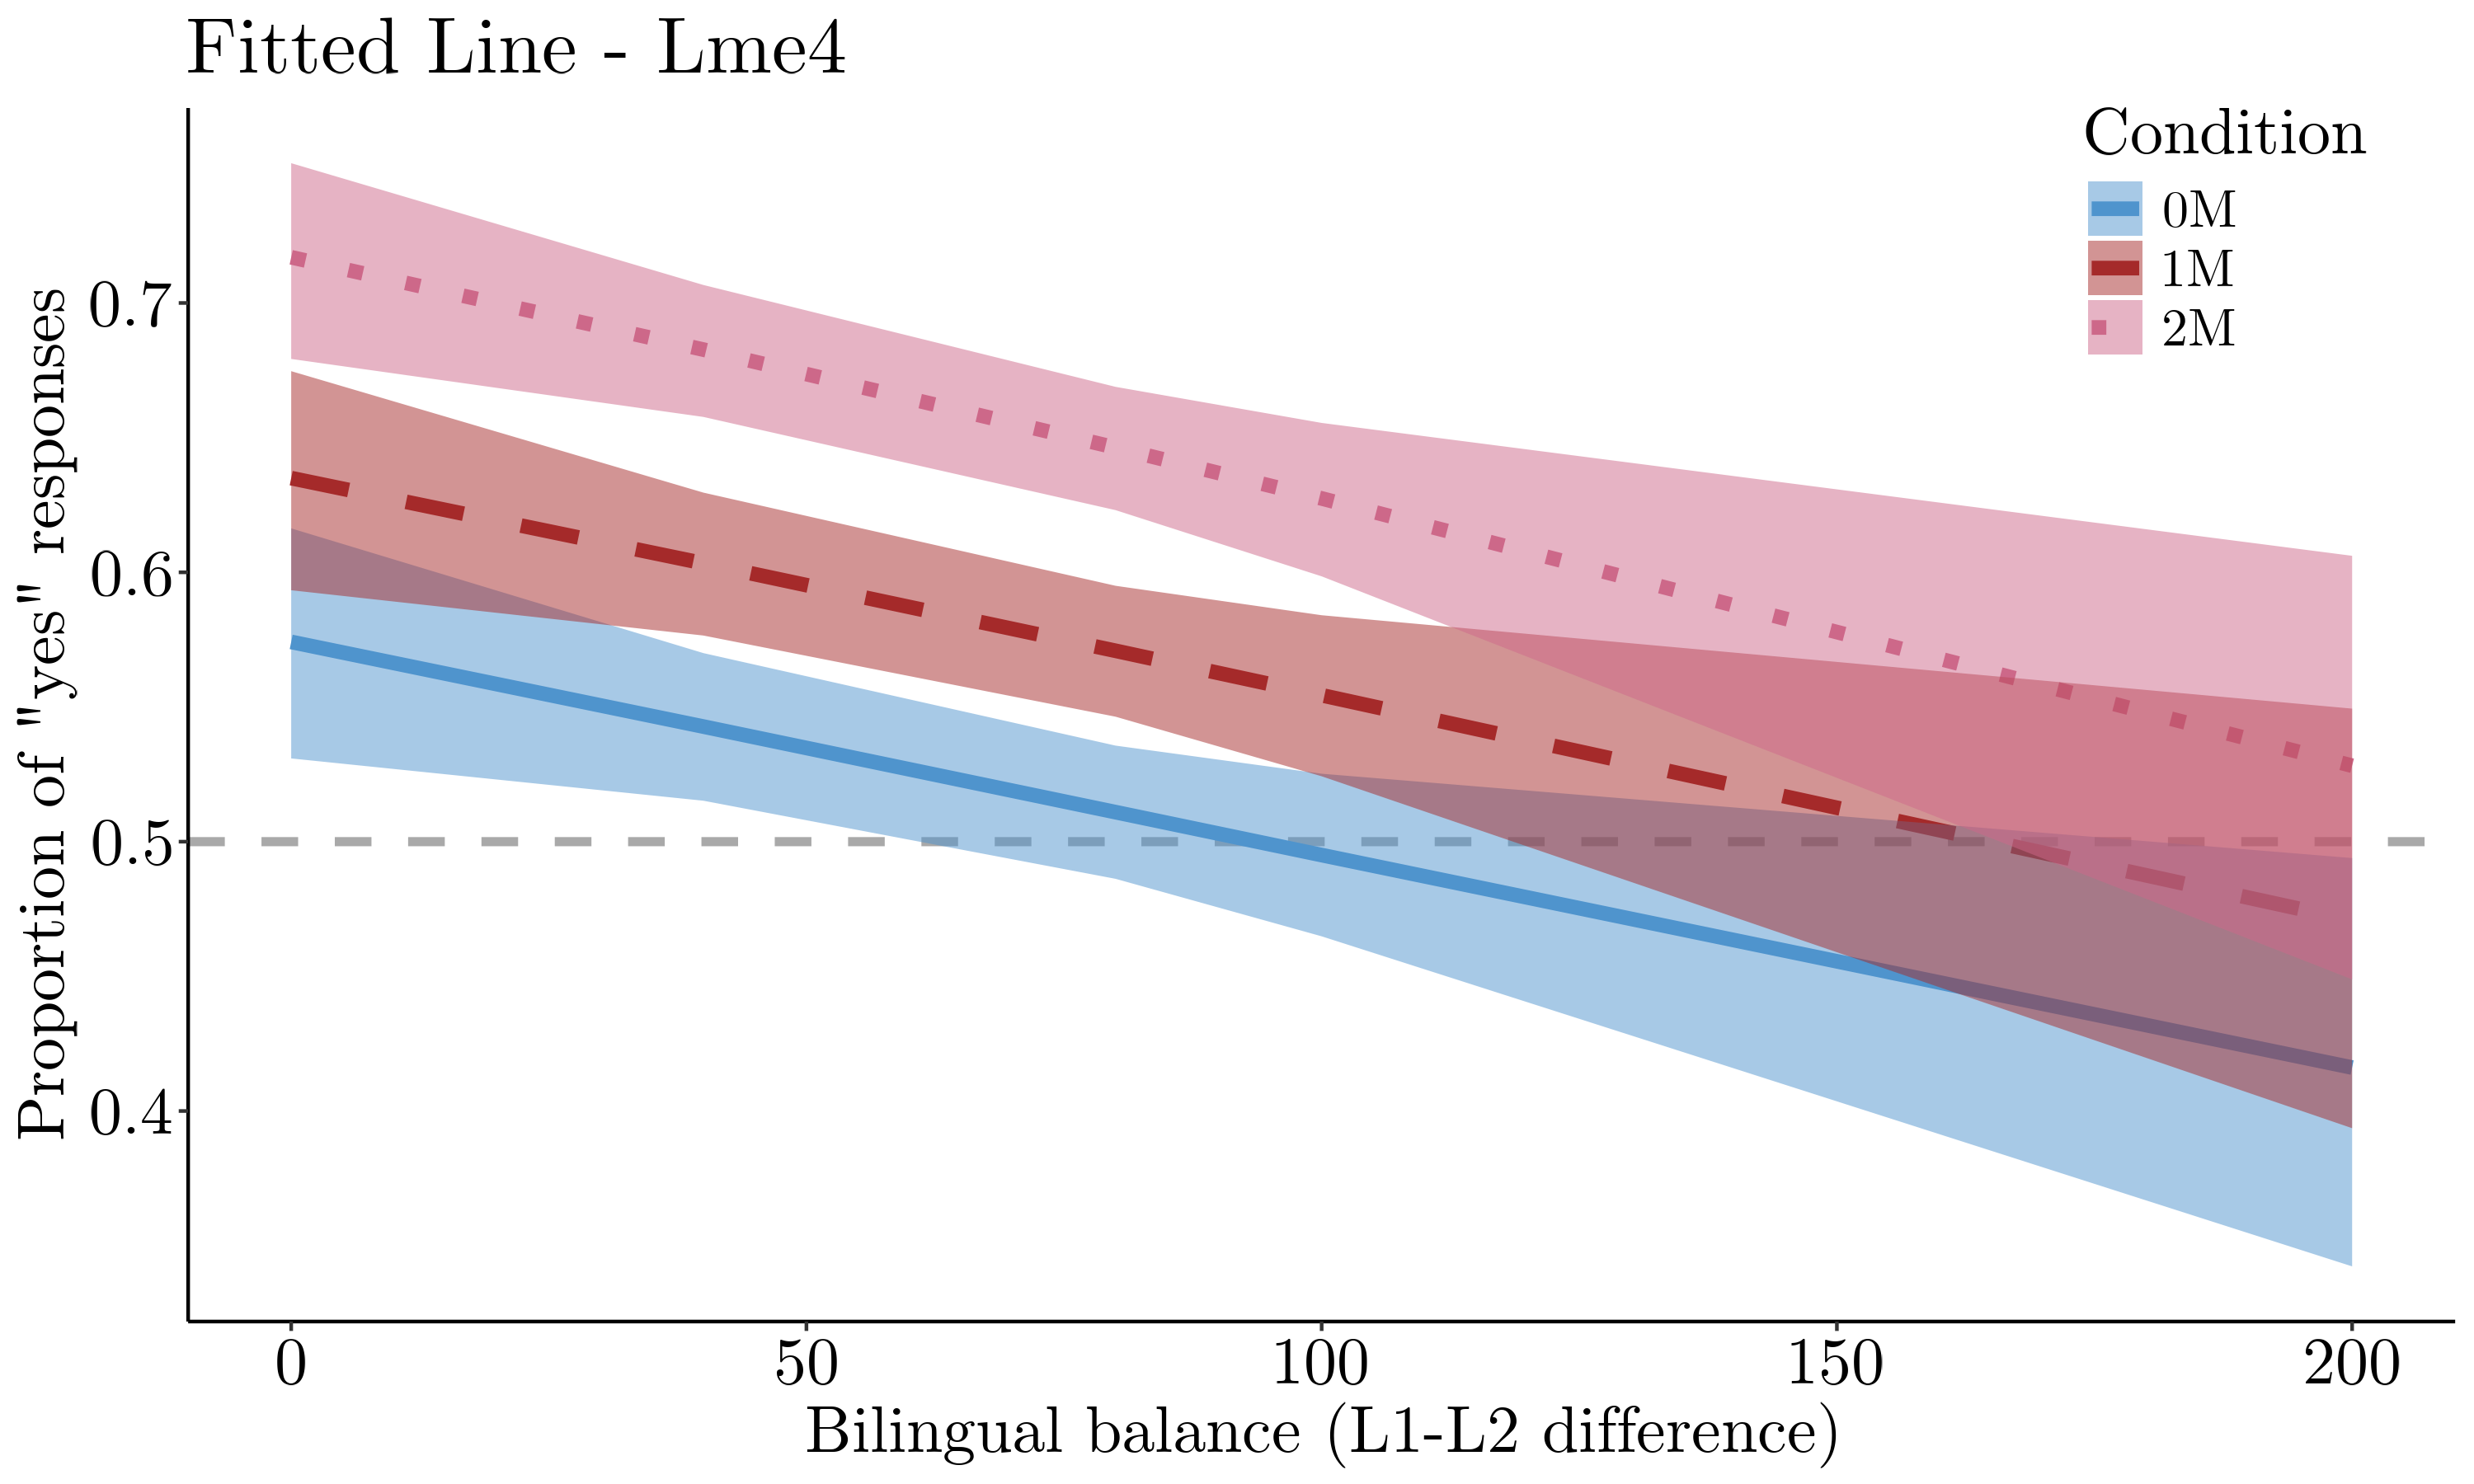
\includegraphics[width=0.99\textwidth]{Figures/Exp2_yes_L1L2diff.png}
    \end{minipage}
    \begin{minipage}{0.49\linewidth}
        \centering
        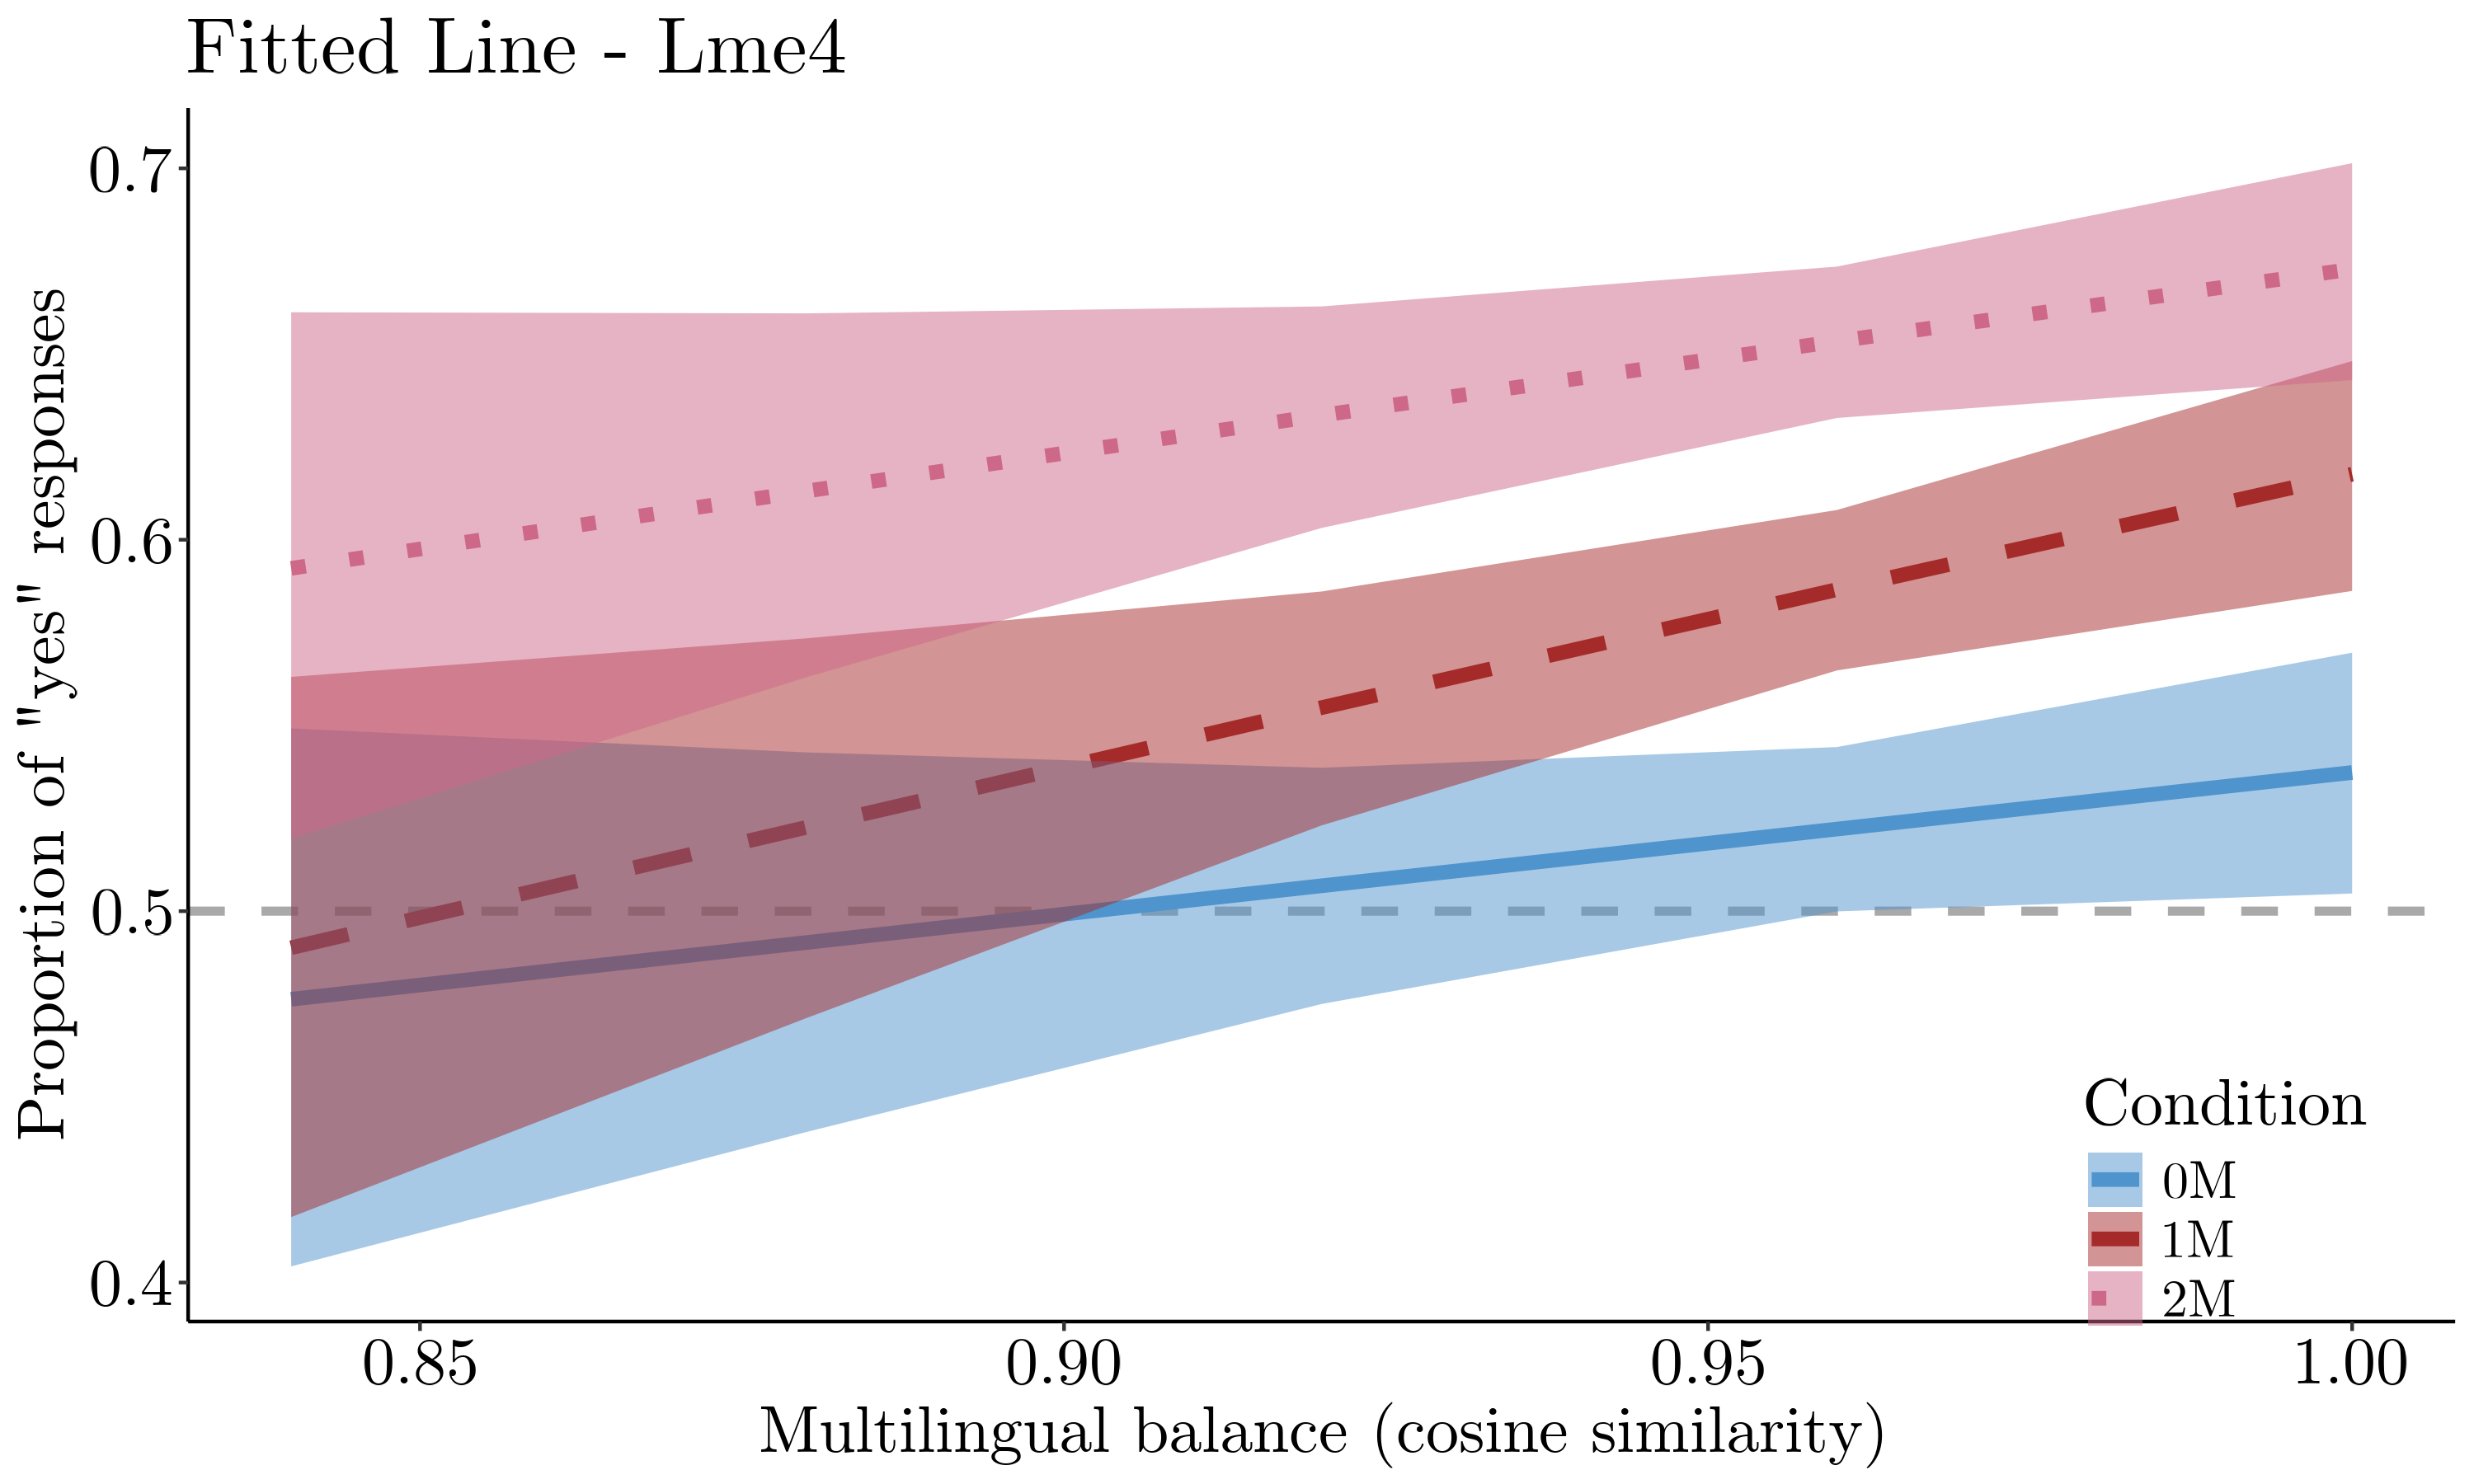
\includegraphics[width=0.99\textwidth]{Figures/Exp2_yes_cossim.png}
    \end{minipage}
    \caption[]{\justifying Model estimates of the effect of PC7 (L2 History; top right), multilingual experience (bottom right), bilingual balance (L1-L2 difference; bottom left), and cosine similarity (bottom right)  on ``yes'' responses, for the 0M (blue), 1M (red), and 2M (pink) conditions. Higher values of PC7 means longer L2 knowledge. L1-L2 difference scores closer to 0 indicate a more balanced bilingual profile. Cosine similarity scores closer to 1 indicate more balance across a participants' languages. Bars around the lines indicate the 95\% confidence interval. Dashed lines at 0.5 indicate chance level.}
    \label{exp2_yes_gender/PC7/multiexp/L1L2diff}
\end{figure}

Other metrics increased the observed morpheme familiarity effect. The distribution of ``yes'' responses across the 0M, 1M, and 2M conditions was more discriminate for older participants ($\beta$ = 0.10, z = 2.01, p = 0.04), and for those who used their L2 more than their L1 (PC2; $\beta$ = 0.10, z = 2.03, p = 0.04).

\begin{figure}[!htbp]
    \begin{minipage}{0.49\linewidth}
        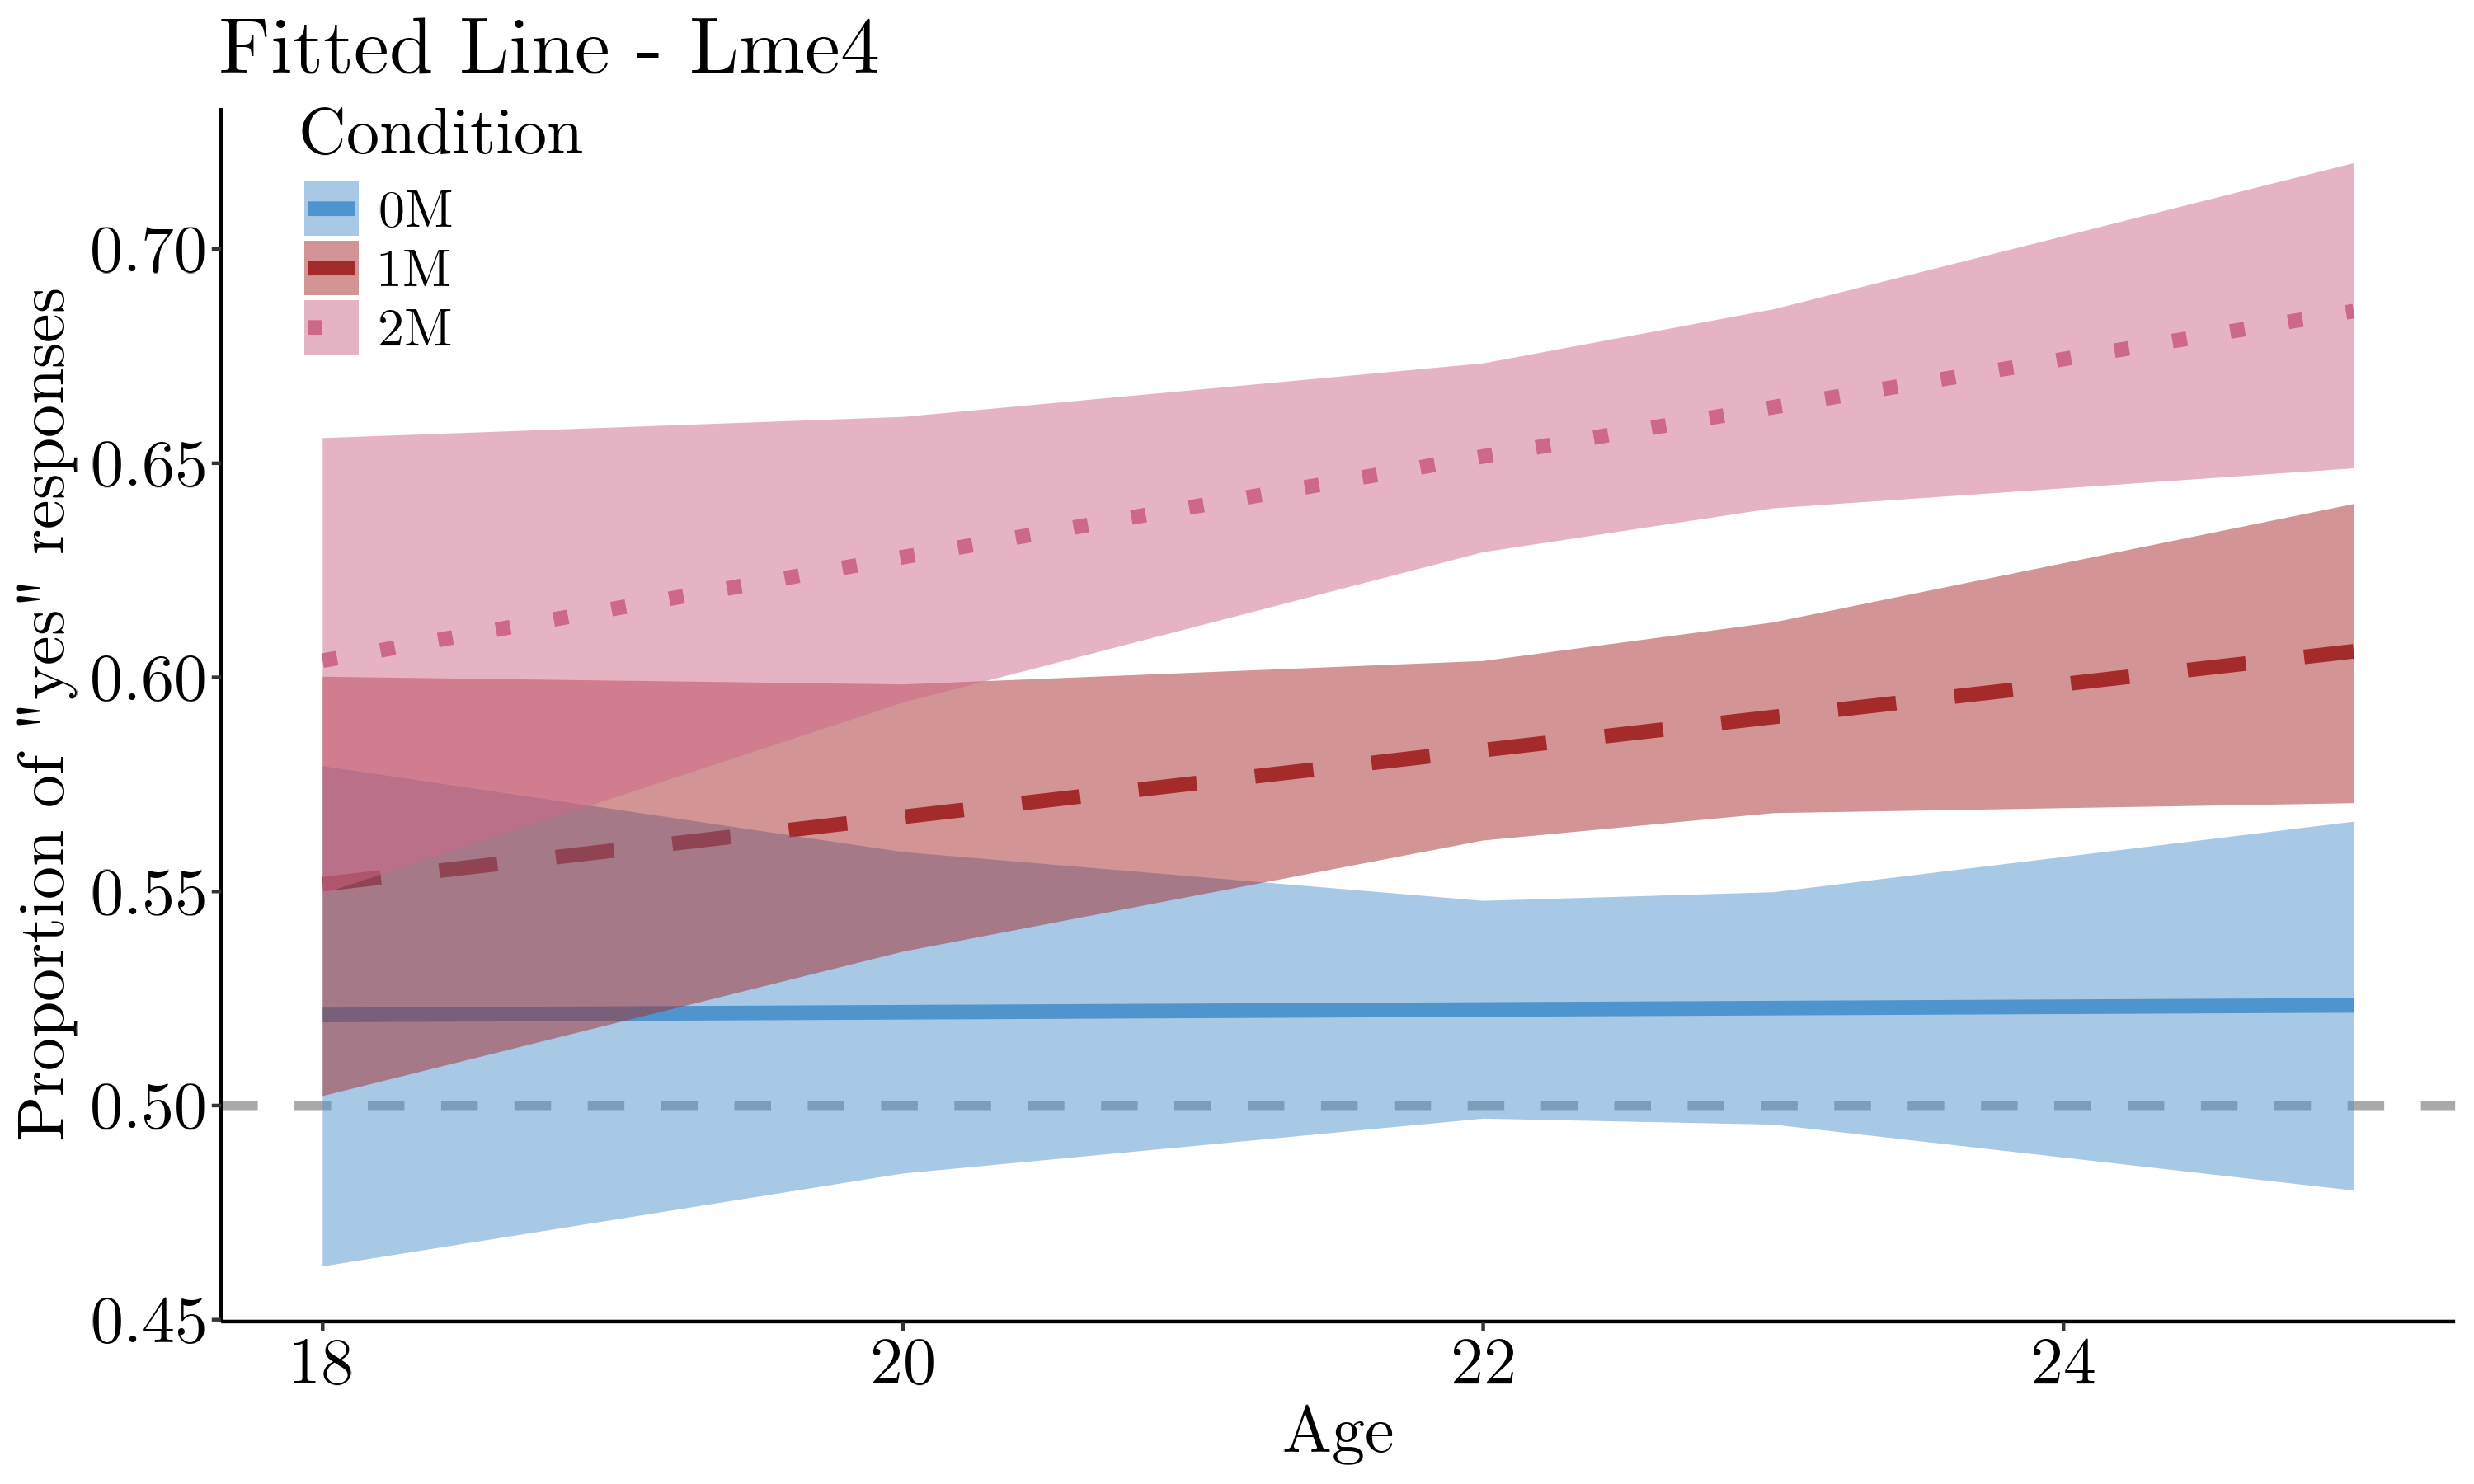
\includegraphics[width=0.99\textwidth]{Figures/Exp2_yes_age.png}
    \end{minipage}
    \begin{minipage}{0.49\linewidth}
        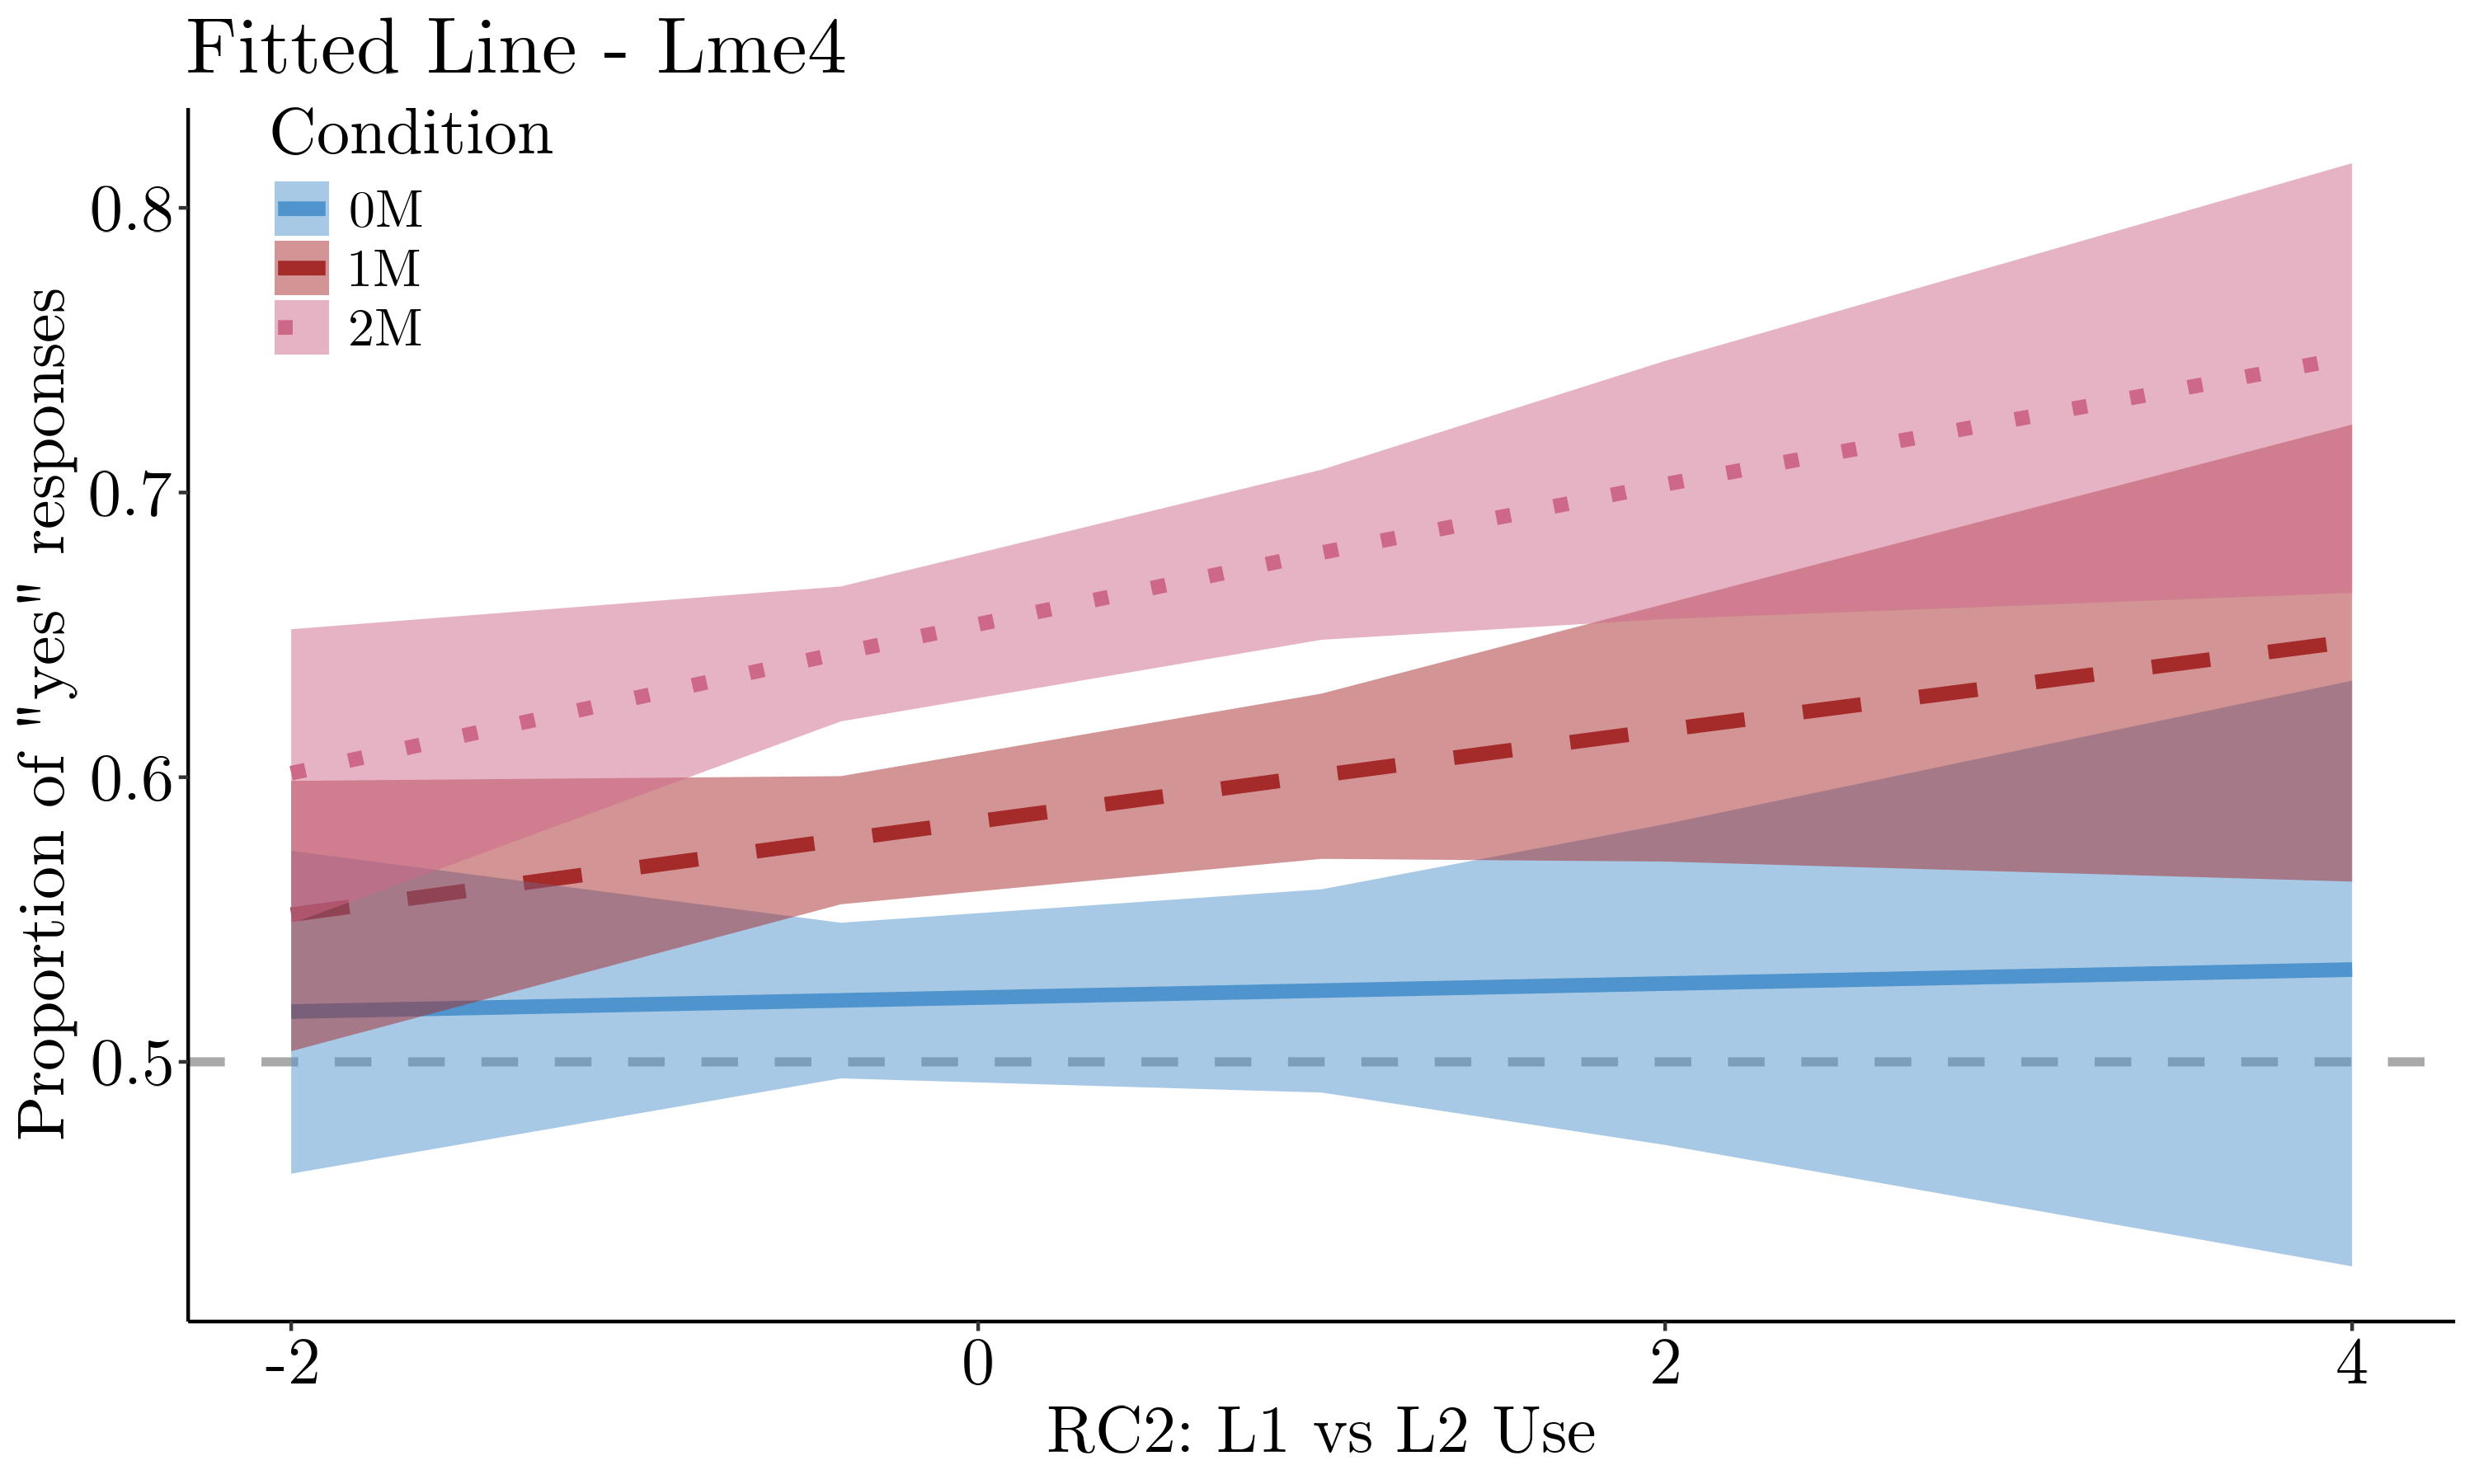
\includegraphics[width=0.99\textwidth]{Figures/Exp2_yes_PC2.png}
    \end{minipage}
    \caption[]{\justifying Model estimates of the effect of age (left) and PC2 (L1 vs L2 use; right) on ``yes'' responses, for the 0M (blue), 1M (red), and 2M conditions (pink). Higher values of PC2 translates to more use of participants' L2 comparatively to their L1. Bars around the lines indicate the 95\% confidence interval. Dashed lines at 0.5 indicate chance level.}
    \label{exp2_yes_age/PC2}
\end{figure}

\begin{table}[!htbp]
    \begin{center}
        \begin{tabular}{@{}lllll@{}}
            \toprule
            \multicolumn{5}{l}{\textbf{``yes'' responses across conditions}} \\ \midrule
            & \textbf{$\beta$} & \textbf{SE} & \textbf{z-value} & \textbf{p-value} \\ \midrule
            PC7 (L2 history) & 0.11 & 0.05 & 2.20 & 0.03 \\ \midrule
            Bilingual balance (L1-L2 difference) & -0.10 & 0.05 & -2.02 & 0.04 \\ \midrule
            Multilingual experience & 0.15 & 0.04 & 3.34 & 0.0008 \\ \midrule
            Multilingual experience$\ast$1M & -0.08 & 0.04 & -2.26 & 0.02 \\ \midrule
            Age$\ast$2M & 0.10 & 0.05 & 2.01 & 0.04 \\ \midrule
            PC2 (L1 vs L2 use)$\ast$2M & 0.10 & 0.05 & 2.03 & 0.04 \\ \bottomrule
        \end{tabular}
    \end{center}
    \caption{Summary of experiment 2 mixed modelling statistics of ``yes'' responses across conditions, for significant variables.}
    \label{exp2_yes_summary}
\end{table}
\break

\noindent
\underline{2M performance}

\noindent
Measures of balance affected the amount of ``yes'' responses to the 2M conditions. Higher levels of bilingual imbalance (according to L1-L2 difference) drove the proportion of ``yes'' responses down ($\beta$ = -0.15, z = -2.69, p = 0.007), and the same was true for multilingual balance (as defined by cosine similarity; $\beta$ = 0.14, z = 2.45, p = 0.01), as can be seen in \autoref{exp2_2Myes}.

\begin{figure}[!htbp]
    \begin{minipage}{0.49\linewidth}
        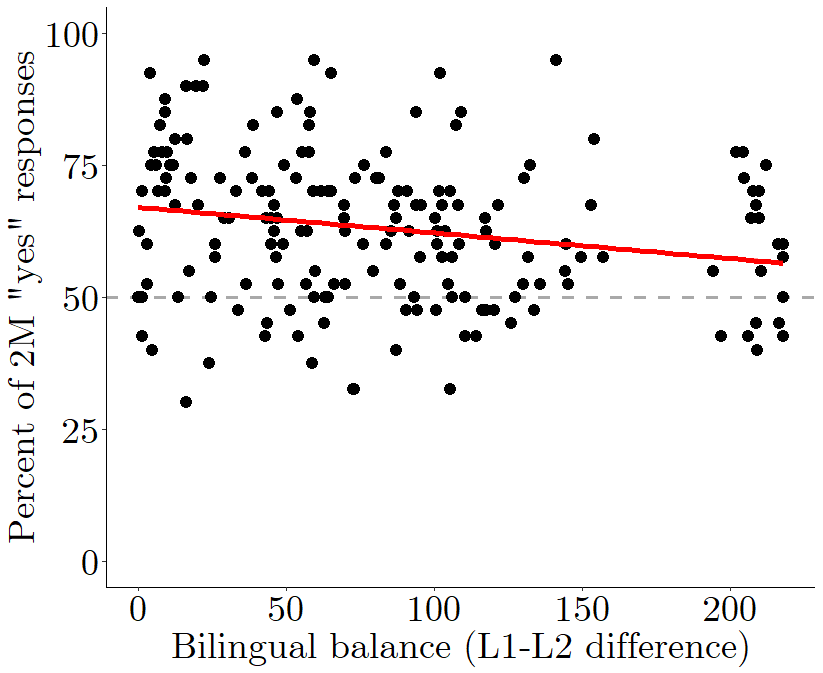
\includegraphics[width=0.99\textwidth]{Figures/Exp2_2Myes_L1L2diff.png}
    \end{minipage}
    \begin{minipage}{0.49\linewidth}
        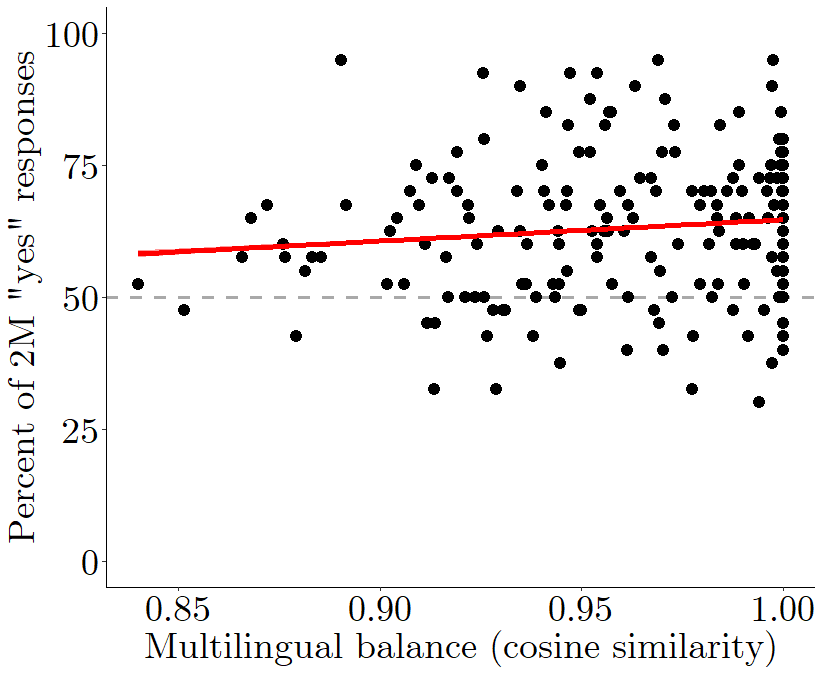
\includegraphics[width=0.99\textwidth]{Figures/Exp2_2Myes_cossim.png}
    \end{minipage}
    \caption[]{\justifying Plots of the percent of ``yes'' responses in the 2M condition as a function of bilingual balance (L1-L2 difference; left) and multilingual balance (cosine similarity; right). Lower levels of L1-L2 difference indicate more balanced profiles, as do higher levels of cosine similarity. Dashed lines at 50\% indicate chance level.}
    \label{exp2_2Myes}
\end{figure}

While quadrilinguals had higher 2M accuracy than monolinguals ($\beta$ = 0.45, z = 2.38, p = 0.02), they were not actually above chance (t(40) = 1.28, p = 0.21; see \autoref{exp2_2Mcategory}). Multilingual balance, or cosine similarity, also initially had a significant interaction with 2M accuracy ($\beta$ = -0.11, z = -2.13, p = 0.03), but this effect was lessened to the extent of non-significance when the monolingual population was removed from analysis ($\beta$ = -0.08, z = -1.42, p = 0.16). Monolinguals are a special case when it comes to multilingual balance, as they necessarily calculate as perfectly balance due to their single data point. This was therefore deemed insufficient evidence in favour of a multilingual balance effect.

\begin{figure}[!htbp]
    \begin{center}
        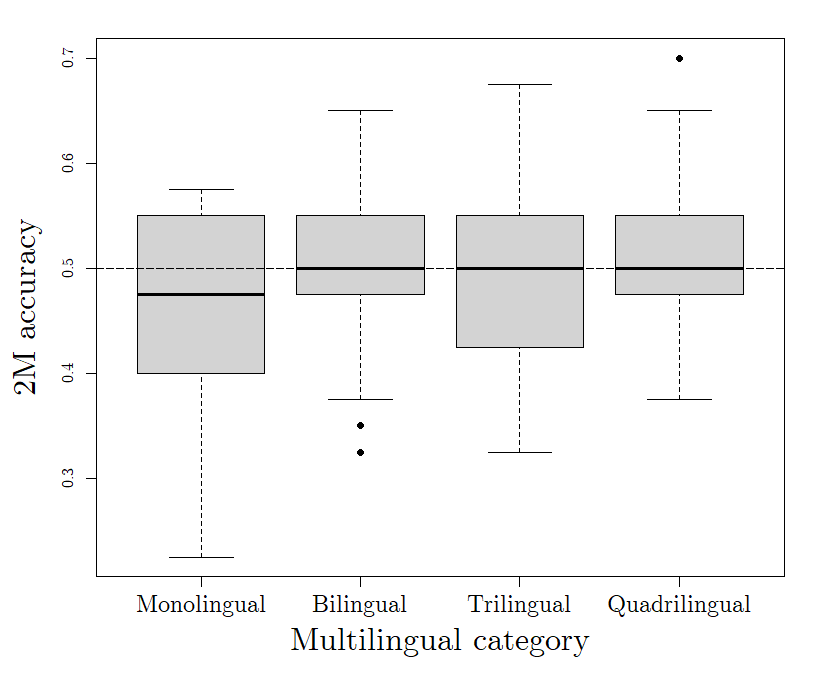
\includegraphics[width=0.6\textwidth]{Figures/Exp2_2M_category.png}
    \end{center}
    \caption[]{\justifying Plot of the relationship between 2M accuracy and multilingual category. The dashed lines indicates chance level.}
    \label{exp2_2Mcategory}
\end{figure}

An interesting relationship between 2M scores and participant language script type was found. Participants who spoke different scripts had 2M scores above chance level (t(27) = 2.10, p = 0.045), with scores estimated around 53\% (\autoref{exp2_2M_script}).

\begin{figure}[!htbp]
    \begin{center}
        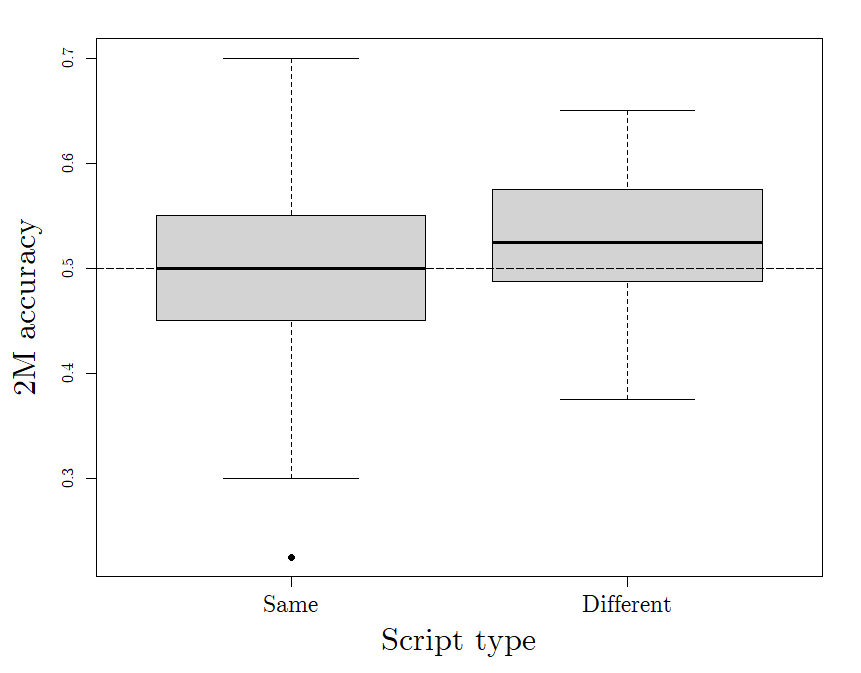
\includegraphics[width=0.6\textwidth]{Figures/Exp2_2M_script.png}
    \end{center}
    \caption[]{\justifying Box plots of 2M accuracy scores for each language script type. The dashed line indicates chance level.}
    \label{exp2_2M_script}
\end{figure}

\begin{table}[!htbp]
    \begin{center}
        \begin{tabular}{@{}lllll@{}}
            \toprule
            \multicolumn{5}{l}{\textbf{2M ``yes'' responses and accuracy}} \\ \midrule
            & \textbf{$\beta$} & \textbf{SE} & \textbf{z-value} & \textbf{p-value} \\ \midrule
            Bilingual balance (L1-L2 difference) & -0.15 & 0.06 & -2.69 & 0.007 \\ \midrule
            Quadrilingual$\ast$correct & 0.45 & 0.19 & 2.38 & 0.02 \\ \midrule
            Different scripts$\ast$correct & 0.32 & 0.15 & 2.12 & 0.03 \\ \bottomrule
        \end{tabular}
    \end{center}
    \caption{Summary of experiment 2 mixed modelling statistics of 2M ``yes'' responses and accuracy across conditions, for significant variables.}
    \label{exp2_2M_summary}
\end{table}
\break